\documentclass[12pt]{article}
\usepackage[margin=0.8in,top=0.8in,bottom=0.8in]{geometry}
\usepackage{graphicx}
\usepackage{wrapfig}
\newcommand \beq {\begin{equation}}
\newcommand \eeq {\end{equation}}
\newcommand \beqn {\begin{eqnarray}}
\newcommand \eeqn {\end{eqnarray}}
\newcommand{\ve}[1]{\mbox{\boldmath $#1$}}

\begin{document}
\title{Doppler Effect and ``Supersonic'' Motion}
\author{Yuk Tung Liu}
\date{2018-01-08}
\maketitle

The theory and method used for the animations are described. Here ``supersonic'' 
simply refers to the source moving at a speed faster than the wave speed.

\section{Mathematical Formulation}

Consider the wave equation 
\beq
  \nabla^2 \psi - \frac{1}{c^2} \frac{\partial^2 \psi}{\partial t^2} 
= -4\pi s(\ve{x},t) ,
\label{eq:wave}
\eeq
where $c$ is the wave speed and $s$ is a source term. The equation can be 
solved using the method of Green's function. The retarded solution 
is given by (see, e.g., Ch.~6 of 
{\it Classical Electrodynamics} by J.D.~Jackson) 
\beq
  \psi(\ve{x},t) = \int \frac{s(\ve{x}',t_r)}{|\ve{x}-\ve{x}'|} d^3 x' ,
\label{eq:psi_solution}
\eeq
where $t_r = t-|\ve{x}-\ve{x}'|/c$ is the retarded time. Consider a point 
source emitting a wave of constant frequency $f$ at its rest frame at 
$t > 0$, and it is moving along a trajectory given by $\ve{x}_s(t)$. 
The source function can be written as 
\beq
  s(\ve{x},t) = A \delta(\ve{x}-\ve{x}_s(t)) e^{-i\omega t} \Theta(t) ,
\label{eq:f}
\eeq
where $\omega = 2\pi f$, $A$ is a constant related to the amplitude of the 
generated waves, $\Theta(t)=0$ for $t<0$ and 1 for $t>0$ is 
the Heaviside step function. The function $\Theta(t)$ is inserted so that 
the source emits waves only after $t>0$.

Substituting Eq.~(\ref{eq:f}) into~(\ref{eq:psi_solution}) yields the following
Li{\'e}nard-Wiechert-like formula:
\beq
  \psi(\ve{x},t) = \frac{A e^{-i\omega t_r}}{|\ve{x}-\ve{x}_s(t_r)| 
[1-\ve{\beta}_s(t_r) \cdot \hat{\ve{n}}(t_r)]} \Theta(t_r) , 
\label{eq:psi}
\eeq
where $\ve{\beta}_s(t_r)=\ve{v}_s(t_r)/c$, $\ve{v}_s(t_r)=\dot{\ve{x}}_s(t_r)$ is the 
velocity of the source at the retarded time, and $\hat{\ve{n}}(t_r)=(\ve{x}-\ve{x}_s(t_r))/
|\ve{x}-\ve{x}_s(t_r)|$. Here we assume that there is only one retarded time $t_r$ 
that satisfies the equation $c(t-t_r)=|\ve{x}-\ve{x}_s(t_r)|$. This is true if 
the source moves slower than the wave speed. If $t_{r1}$ and $t_{r2}$ are solutions 
of the equation and $t_{r2}>t_{r1}$, we have 
\beq
  c(t-t_{r1})=|\ve{x}-\ve{x}_s(t_{r1})| \ \ , \ \ 
  c(t-t_{r2})=|\ve{x}-\ve{x}_s(t_{r2})| .
\eeq
Subtracting the two equations yields 
\beq
  c(t_{r2}-t_{r1})=|\ve{x}-\ve{x}_s(t_{r1})| - |\ve{x}-\ve{x}_s(t_{r2})| .
\eeq
Since 
\beq
  |\ve{A}|-|\ve{B}| = \sqrt{(|\ve{A}|-|\ve{B}|)^2} = 
  \sqrt{|\ve{A}|^2 + |\ve{B}|^2 - 2 |\ve{A}||\ve{B}|} \leq 
  \sqrt{|\ve{A}|^2 + |\ve{B}|^2 - 2 \ve{A}\cdot \ve{B}} = |\ve{A}-\ve{B}| ,
\eeq
it follows that 
\beq
  c(t_{r2}-t_{r1}) \leq |\ve{x}_s(t_{r2})-\ve{x}_s(t_{r1})| \ \ \Rightarrow \ \ 
  \frac{|\ve{x}_s(t_{r2})-\ve{x}_s(t_{r1})|}{t_{r2}-t_{r1}} \geq c .
\eeq
This means that the average speed of the source in the time interval $(t_{r1},t_{r2})$ 
is faster than the wave speed. So multiple retarded times can only occur if $v_s \geq c$. 
In the case of multiple retarded times, $\psi$ is given by the sum of contributions 
from these retarded times.

A special case is when the source is stationary: $\ve{x}_s=0$ at all time. 
Then $t_r=t-r/c$, where $r=|\ve{x}|$ is the distance from the source. Equation~(\ref{eq:psi}) 
becomes 
\beq
  \psi(\ve{x},t) = \frac{A e^{i(kr-\omega t)}}{r} \Theta \left(t-\frac{r}{c}\right) ,
\eeq
where $k=\omega r/c$. This solution describes an outgoing spherical wave.

\section{Animation Setup}

The animation is based on Eq.~(\ref{eq:psi}). For a given point $\ve{x}$, the 
wave function $\psi$ is obtained by finding the retarded position of the source and 
then apply Eq.~(\ref{eq:psi}). We can turn it around and consider a time
sequence $t_1<t_2<\cdots < t_n$. At any given time $t \geq t_n$, a wave emitted at time
$t_i$ reaches a spherical surface of radius $c(t-t_i)$ centered at $\ve{x}_s(t_i)$. 
The retarded time for points on this sphere is $t_i$ and the wave function of 
points on this 
sphere is $A e^{-i\omega t_i}/[c(t-t_i) (1-\ve{\beta}(t_i)\cdot \hat{\ve{n}}(t_i))]$. 

The simplest choice of the time sequence $\{t_i\}$ is $t_i=i/f$, (($i=0, 1, 2,\cdots$). 
In this case, the phase of the wave at these $t_i$ are the same and the spheres 
$\{S_i: |\ve{x}-\ve{x}_s(t_i)| = c(t-t_i)\}$ are the wavefronts.

The procedure for creating the animation is very simple: 

1. For any given time $t>0$, calculate $n=[tf]$, where $[x]$ denotes the largest 
integer smaller than $x$. The value of $n$ is the number of times $t_i$ in the 
time sequence so far.

2. For each $i\in [0,n]$, draw a circle of radius $c(t-t_i)$ centered at $\ve{x}_s(t_i)$. 
A circle is drawn instead of a sphere to make the animation two-dimensional. The $n$ 
circles represent the wavefronts.

3. Draw the source position at $\ve{x}_s(t)$.

An animation is produced by generating a new picture at different $t$ every 20~ms. 
The procedure is intuitive. It simply says a wavefront generated at time $t_i$ 
spreads out from the source at the wave speed. The distance between the successive 
wavefront is the wavelength. Since the wave speed is constant, the wavelength at 
a given point is inversely proportional to the observed frequency. The observed 
frequency at a given point can also be measured by counting the number of wavefronts 
passing through the point per unit time. 

It is also easy to see that when the source speed $v_s <c$ at all times, the 
retarded time at any point is unique since a wave emitted at $t_i$ is always 
inside a sphere of the wave generated at $t<t_i$, so the spheres never cross. 
However, if $v_s>c$, a wave emitted at $t_i$ is outside the sphere of a wave generated 
at a slightly earlier time and the two spheres will cross as they expand. 
When that happens, the 
intersection points will have two different retarded times.

We consider two cases of $\ve{x}_s(t)$ in the animation page. The first case is 
a motion with constant velocity in which $\ve{x}_s(t)=\ve{v} t$. In the second case 
the source moves in a circle of radius $r_s$ with constant speed $v_s$ in which 
$\ve{x}_s(t) = r(\cos \Omega t \hat{\ve{x}} + \sin \Omega t \hat{\ve{y}})$.
Here $\Omega = v_s/r_s$.

\section{Doppler Effect: Moving Source vs Moving Observer}

It follows from Eq.~(\ref{eq:psi}) that the phase of the wave is 
\beq
  \phi(\ve{x},t) = \phi_A - \omega t_r(\ve{x},t) ,
\eeq
where $\phi_A$ is the phase of the constant $A$: $A=|A|e^{i\phi_A}$.
The observed angular frequency is 
\beq
  \omega_{\rm obs} = \left| \frac{d\phi}{dt}\right| = \omega \frac{dt_r}{dt} .
\label{eq:omg_obs1}
\eeq
Let $\ve{x}_{\rm obs}(t)$ be the observer's position as a function of $t$. 
Then $t_r = t-|\ve{x}_{\rm obs}(t)-\ve{x}_s(t_r)|/c$ and 
\beqn
  \frac{dt_r}{dt} &=& 1 - \frac{1}{c} \frac{d}{dt} |\ve{x}_{\rm obs}(t)-\ve{x}_s(t_r)| \\ 
&=& 1-\frac{1}{c} \left[ \dot{\ve{x}}_{\rm obs}(t) \cdot \ve{\nabla}_{\ve{x}_{\rm obs}}|\ve{x}_{\rm obs}(t)-\ve{x}_s(t_r)| 
+ \frac{d \ve{x}_s(t_r)}{dt} \cdot \ve{\nabla}_{\ve{x}_s} |\ve{x}_{\rm obs}(t)-\ve{x}_s(t_r)| 
\right] \\ 
&=& 1 - \frac{1}{c} \left[ \ve{v}_{\rm obs}(t) \cdot \hat{\ve{n}}(t_r) -\frac{dt_r}{dt} \dot{\ve{x}}_s(t_r) \cdot \hat{\ve{n}}(t_r)\right] \\ 
&=& 1 - \frac{1}{c} \left[ \ve{v}_{\rm obs}(t) \cdot \hat{\ve{n}}(t_r) 
- \frac{dt_r}{dt} \ve{v}_s(t_r) \cdot \hat{\ve{n}}(t_r) \right] 
\eeqn
\beqn
\Rightarrow \ \ \left(1-\frac{\ve{v}_s(t_r) \cdot \hat{\ve{n}}(t_r)}{c}\right)\frac{dt_r}{dt} 
&=& 1- \frac{\ve{v}_{\rm obs}(t) \cdot \hat{\ve{n}}(t_r)}{c}  \\ 
\Rightarrow \ \ 
\frac{dt_r}{dt} &=& \frac{1-\ve{\beta}_{\rm obs}(t) \cdot \hat{\ve{n}}(t_r)}
{1-\ve{\beta}_s(t_r) \cdot \hat{\ve{n}}(t_r)} ,
\label{eq:dtr_dt}
\eeqn
where $\hat{\ve{n}}(t_r) = [\ve{x}_{\rm obs}(t)-\ve{x}_s(t_r)]/|\ve{x}_{\rm obs}(t)-\ve{x}_s(t_r)|$, 
$\ve{\beta}_{\rm obs}=\ve{v}_{\rm obs}/c$, $\ve{\beta}_s=\ve{v}_s/c$, 
and all velocities are measured relative to the rest frame of the medium in which 
the waves propogate. Combining Eqs.~(\ref{eq:dtr_dt}) and (\ref{eq:omg_obs1}) yields 
\beq
\omega_{\rm obs}(t) = \frac{1-\ve{\beta}_{\rm obs}(t) \cdot \hat{\ve{n}}(t_r)}
{1-\ve{\beta}_s(t_r) \cdot \hat{\ve{n}}(t_r)}\, \omega \ .
\label{eq:omg_obs_general}
\eeq

Equation~(\ref{eq:omg_obs_general}) is a general formula of the Doppler shift 
when both the source and observer are moving relative to the medium. 
If the observer is stationary, 
$\ve{\beta}_{\rm obs}=0$ and the equation reduces to 
\beq
  \omega_{\rm obs}(t) = \frac{\omega}{1-\ve{\beta}_s(t_r) \cdot \hat{\ve{n}}(t_r)} \ .
\label{eq:Doppler_moving_source}
\eeq
For a stationary source, $\ve{\beta}_s=0$ and the equation reduces to 
\beq
  \omega_{\rm obs}(t) = \omega [1-\ve{\beta}_{\rm obs}(t) \cdot \hat{\ve{n}}(t_r)] .
\label{eq:Doppler_moving_observer}
\eeq
These two formulae can also be derived easily using a geometric approach. 
The difference between a moving source and a moving observer is that for a 
moving source, the wave speed is the same in every direction but the wavelength 
depends on the direction: compressed in the direction of the source's motion 
and expanded in the opposite direction. In the case of a moving observer and 
stationary source, the wavelengths are the same everywhere but the wave speed 
is anisotropic in the observer's rest frame.

Although the two formulae both imply that the observed frequency increases (decreases) 
when the source is moving towards (away from) the observer, the 
amount of shift is slightly different. However, both formulae give the same 
result to first order in $v/c$ when $v \ll c$. Note that this analysis cannot 
be applied to light since light does not propagate through a medium. The Doppler 
shift of light depends only on the relative velocity between the source and 
observer.

In the case of a stationary observer and moving source, the wave speed is 
unchanged. The change in frequency means that the wavelength changes. In particular, 
the wavelength is multiplied by a factor $1-\ve{\beta}_s(t_r) \cdot \hat{\ve{n}}$ 
compared to the wavelength emitted by a stationary source. On the other hand, 
equation~(\ref{eq:psi}) implies that the amplitude of the wave also changes as 
a result of the source's motion: the amplitude is multiplied by a factor 
$1/[1-\ve{\beta}_s(t_r) \cdot \hat{\ve{n}}]$, which is exactly the inverse of the 
wavelength factor. This means that the density of the wavefront observed in an animation 
is proportional to the enhancement factor of the wave amplitude.

\section{Motion with $\ve{v_s > c}$}

One important feature of $v_s>c$ motion is the presence of a shock wave. This 
can be seen from equation~(\ref{eq:psi}). When $v_s>c$, there is a direction $\hat{\ve{n}}$ 
in which $\ve{\beta}_s \cdot \hat{\ve{n}}=1$ and $\psi$ is singular in that direction. 
In many cases, the wave equation~(\ref{eq:wave}) arises from a linear perturbation 
analysis. 
When the amplitude of the wave becomes large, the wave equation is no longer valid and 
nonlinear effects must be taken into account. The shock structures for the constant 
velocity motion and circular motion are analyzed below.

\subsection{Constant Velocity Motion}

\begin{figure}[h]
%\vskip -4mm
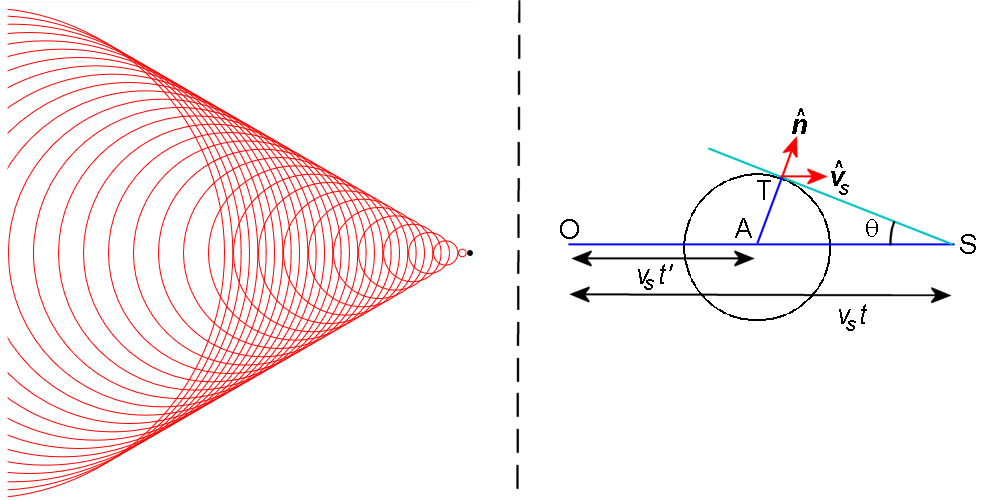
\includegraphics[width=14cm]{MachCone.png}
\caption{Left: Bow wave generated by a source (represented by a black dot) 
moving with constant velocity $v_s=2c$ to the right. Red lines are wavefronts 
of waves generated at earlier times. Right: The geometry of the Mach cone.}
\label{fig:bow_wave}
\end{figure}

For the constant-velocity motion, the shock wave forms the well-known Mach cone 
as shown on the left side of Figure~\ref{fig:bow_wave}. 
This is also known as a bow wave, often seen when a ship moves through 
the water. The geometry of the Mach cone is shown on the right side of Figure~\ref{fig:bow_wave}. 
At $t=0$, the source is at point $O$. At time $t$, the source moves to point $S$, which 
is at a distance $v_s t$ to the right of $O$. Consider the wave emitted at time $t'<t$ when 
the source is at point $A$, a distance $v_s t'$ to the right of $O$. At time $t$, the 
wavefront of the wave emitted at $t'$ is a sphere of radius $c(t-t')$ centered 
at $A$. Consider a point $T$ on the sphere at which the line ST is tangent to the 
sphere. From the figure, the angle $\theta$ is given by 
\beq
  \sin \theta = \frac{|\overline{AT}|}{|\overline{AS}|} = \frac{c(t-t')}{v_s(t-t')} 
 = \frac{c}{v_s} .
\eeq
Note that this angle is the same for all $0 \leq t' < t$. Hence the tangent points of the 
spheres form a cone with vertex at $S$ and the axis along $-\ve{v}_s$. The angle 
of the cone from the axis is $\theta = \sin^{-1}(c/v_s)$. This is known as the Mach cone.
It is easy to show that 
$\ve{\beta}_s(t_r) \cdot \hat{\ve{n}}=\beta_s \sin \theta = 1$ at $T$. Thus the 
shock wave is on the Mach cone. In the case a supersonic aircraft, 
a thud is heard when the shock wave passes through an observer. This is known as the 
sonic boom. 

Another way to find the surface on which the shock wave lives at time $t$ is to 
gather all singular points emitted at time $\lambda < t$. It is useful to go through 
the algebra here since the same analysis will be used to study the shock 
structure in the circular motion case. 
Given any direction $\hat{\ve{m}}$, the wave emitted at time $\lambda < t$ reaches the 
position 
\beq
  \ve{x}(\hat{\ve{m}},\lambda) = \ve{x}_s(\lambda) + c(t-\lambda) \hat{\ve{m}} .
\label{eq:xmlambda}
\eeq
Shocks propagate along the direction in which $\hat{\ve{m}}\cdot \ve{\beta}_s=1$ or 
$\hat{\ve{m}}\cdot \hat{\ve{\beta}}_s=1/\beta_s$. We can write 
\beq
  \hat{\ve{m}} =\frac{1}{\beta_s} \hat{\ve{\beta}}_s + 
\frac{\sqrt{\beta_s^2-1}}{\beta_s} \hat{\ve{\beta}}_{s\perp} 
\label{eq:mshock}
\eeq
with $\hat{\ve{\beta}}_{s\perp} \cdot \hat{\ve{\beta}}_s=0$. For constant-velocity motion, 
we can set $\hat{\ve{\beta}}_s=\hat{\ve{x}}$ and 
$\hat{\ve{\beta}}_{s\perp}=\cos \varphi \hat{\ve{y}} + \sin \varphi \hat{\ve{z}}$ with 
$\varphi \in [0,2\pi)$. Then the shock direction is given by 
\beq
 \hat{\ve{m}}_{\rm shock} = \frac{1}{\beta_s} \hat{\ve{x}} + 
\frac{\sqrt{\beta_s^2-1}}{\beta_s} (\cos \varphi \hat{\ve{y}} + \sin \varphi \hat{\ve{z}}) 
\eeq
and the location of the shock at time $t$ is 
\beqn
  \ve{x}_{\rm shock}(\varphi,\lambda) &=& v_s \lambda \hat{\ve{x}} + 
\frac{c(t-\lambda)}{\beta_s}\hat{\ve{x}} + c(t-\lambda) \frac{\sqrt{\beta_s^2-1}}{\beta_s} 
(\cos \varphi \hat{\ve{y}} + \sin \varphi \hat{\ve{z}}) \\ 
&=& v_s t \hat{\ve{x}} + c(t-\lambda)\frac{\beta_s^2-1}{\beta_s}\left[ -\hat{\ve{x}} 
+ \frac{1}{\sqrt{\beta_s^2-1}}(\cos \varphi \hat{\ve{y}} + \sin \varphi \hat{\ve{z}})\right] 
\eeqn
for $\lambda \in [0,t]$ and $\varphi \in [0,2\pi)$. It is straightforward to show that 
the surface is a cone with vertex at $\ve{x}=\ve{x}_s(t)=v_s t\hat{\ve{x}}$. The axis of 
the cone is along $-\hat{\ve{x}}$ ($=-\hat{\ve{v}}_s$) direction and the angle of the cone to the axis 
is $\theta = \tan^{-1}(1/\sqrt{\beta_s^2-1})=\sin^{-1}(1/\beta_s)$. This is precisely 
the Mach cone.

We can see from Figure~\ref{fig:bow_wave} that no waves can reach outside the Mach cone. 
Inside the Mach cone, there is a region in which two wavefronts cross, indicating that 
those are points with two retarded times. The phenomenon can be explained from the equation 
of the retarded time $c(t-t_r)=|\ve{x}-\ve{x}_s(t_r)|$. For constant-velocity motion, 
$\ve{x}_s(t_r)=\ve{v}_s t_r$ and the equation becomes 
\beq
  c(t-t_r) = |\ve{x}-\ve{v}_s t_r| .
\label{eq:tr_constant_v1}
\eeq
It is convenient to consider the transformation $u=c(t-t_r)$ and $\ve{q}=\ve{x}-\ve{v}_st$. 
The vector $\ve{q}$ is the position vector measured from the current source position 
$\ve{x}_s(t)$. Equation~(\ref{eq:tr_constant_v1}) becomes 
\beq
  u = |\ve{q}+\ve{\beta}_s u| .
\eeq
Squaring both sides gives 
\beq
   u^2= |\ve{q}+\ve{\beta}_s u|^2 = q^2 + \beta_s^2 u^2 + 2\ve{q}\cdot \ve{\beta}_s ,
\label{eq:tr_constant_v2}
\eeq
which can be simplified to 
\beq
  (1-\beta_s^2)u^2 - 2 \ve{q}\cdot \ve{\beta}_s u - q^2 = 0  .
\eeq
The solution to this quadratic equation is 
\beq
  c(t-t_r) = u= \frac{\ve{q}\cdot \ve{\beta}_s \pm \sqrt{(\ve{q}\cdot \ve{\beta}_s)^2 
+ (1-\beta_s^2)q^2}}{1-\beta_s^2}
\label{eq:tr_constant_v3}
\eeq
Clearly when $\beta_s<1$ (i.e.\ $v_s<c$), there are two solutions: 
one with $t_r<t$ and the other with $t_r>t$. The one with 
$t_r<t$ is the solution to Eq.~(\ref{eq:tr_constant_v1}). 
The one with $t_r>t$ is the solution to the equation $c(t_r-t)=|\ve{x}-\ve{v}_s t_r|$, 
which also gives rise to Eq.~(\ref{eq:tr_constant_v2}) upon squaring. Hence only 
the solution with $t_r<t$ is the retarded time. This is consistent with our earlier 
analysis.

When $\beta_s>1$, solutions only exist if $(\ve{q}\cdot \ve{\beta}_s)^2 +(1-\beta_s^2)q^2\geq 0$, 
which is equivalent to 
\beq
  (\hat{\ve{q}}\cdot \hat{\ve{\beta}}_s)^2 \geq \frac{\beta_s^2-1}{\beta_s^2}
\eeq
\beq
\ \ \ \Rightarrow \ \ 
  \hat{\ve{q}}\cdot \hat{\ve{\beta}}_s \leq -\frac{\sqrt{\beta_s^2-1}}{\beta_s} 
\ \ {\rm or} \ \ 
  \hat{\ve{q}}\cdot \hat{\ve{\beta}}_s \geq \frac{\sqrt{\beta_s^2-1}}{\beta_s} .
\eeq

\begin{wrapfigure}{r}{5cm}
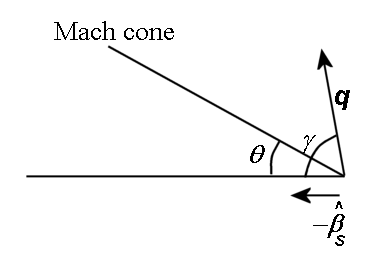
\includegraphics[width=5cm]{MachCone-inout.png}
\caption{\ve{q} is inside or on the Mach cone if the angle $\gamma \leq \theta$.}
\label{fig:MachConeInOut}
\end{wrapfigure}

When $\hat{\ve{q}}\cdot \hat{\ve{\beta}}_s \geq \sqrt{\beta_s^2-1}/\beta_s$, all two 
solutions give $t_r>t$. Hence they are not solutions to Eq.~(\ref{eq:tr_constant_v1}). 
Therefore, Equation~(\ref{eq:tr_constant_v1}) has solutions only when 
\beq
  -\hat{\ve{q}}\cdot \hat{\ve{\beta}}_s \geq \frac{\sqrt{\beta_s^2-1}}{\beta_s} .
\label{eq:cond_solution}
\eeq
This is actually the condition that $\ve{q}$ must be inside or on the Mach cone. 
As shown in Figure~\ref{fig:MachConeInOut}, the vector $\ve{q}$ is inside or on 
the Mach cone only if the angle $\gamma \leq \theta$, where $\theta=\sin^{-1} (1/\beta_s)$ 
is the Mach angle. Since the cosine function is decreasing for angles between 0 and $\pi$, 
the condition $\gamma \leq \theta$ is equivalent to $\cos \gamma \geq \cos \theta$. Since 
$\cos \gamma = \hat{\ve{q}} \cdot (-\hat{\ve{\beta}}_s)$ and $\cos \theta = \sqrt{1-\sin^2 \theta}=
\sqrt{\beta_s^2-1}/\beta_s$, the condition is equivalent to 
$\hat{\ve{q}}\cdot \hat{\ve{\beta}}_s \leq -\sqrt{\beta_s^2-1}/\beta_s$, which is precisely 
Eq.~(\ref{eq:cond_solution}). 

Inside the Mach cone, equation~(\ref{eq:tr_constant_v3}) gives two valid solutions 
for the retarded time $t_r$. We can see from Figure~\ref{fig:bow_wave} that there is 
region in which wavefronts cross. One wavefront corresponds to the retarded position 
$\ve{x}_s(t_r)$ from the left and the other corresponds to the retarded position 
from the right. However, there is also a region where there is only one wavefront 
inside the Mach cone but equation~(\ref{eq:tr_constant_v3}) indicates that there are 
always exactly two values of $t_r$ inside the Mach cone. The reason why we don't see 
two wavefronts in certain region is also clear from the animation. The wave source 
is only on at $t \geq 0$ and the one-wavefront region corresponds to the second 
solution having $t_r<0$ and it doesn't contribution to wave function because no 
wave was generated at $t_r<0$. Mathematically, the vanishing wave function 
at $t_r<0$ is imposed by the step function $\Theta(t_r)$ in Eq.~(\ref{eq:psi}). 

\subsection{Circular Motion}

In this case, the source moves in a circular trajectory with constant speed $v_s$. 
Orient the coordinates so that the source moves in the $x$-$y$ plane and is on the 
positive $x$-axis at $t=0$. The source position can be written as 
\beq
  \ve{x}_s(t) = r_s(\cos \Omega t \hat{\ve{x}} + \sin \Omega t \hat{\ve{y}}) ,
\eeq
where the radius $r_s$ is constant and $\Omega=v_s/r_s$.

\begin{wrapfigure}{r}{7cm}
\vskip -5mm
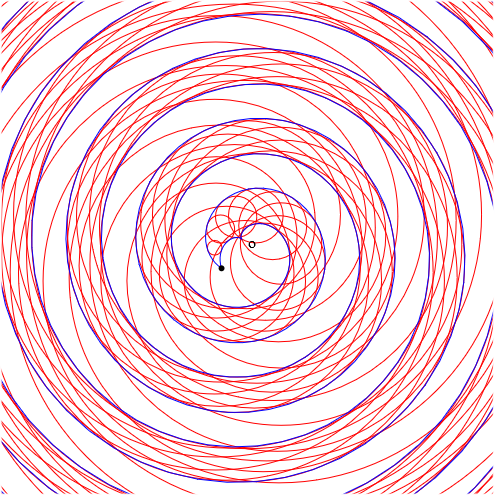
\includegraphics[width=7cm]{circular3c.png}
\caption{Waves generated by a source (represented by a black dot) moving in 
a circle with $v_s=3c$. The center 
of the circilar motion is marked by ``o'' and blue lines are the location of the shock 
wave in the $x$-$y$ plane.}
\label{fig:circular3c}
\vskip 5mm
\end{wrapfigure}

As shown in Figure~\ref{fig:circular3c}, the shock structure of a circular motion 
is more complicated than that of the constant-velocity motion. However, the region 
near the center of the circular motion is relatively simple. Since shock wave propagates 
out along a cone with angle $\alpha = \cos^{-1} (c/v_s)$ from the velocity vector 
$\ve{v}_s$, $\alpha < \pi/2$ and so the shock wave can never reach the center, which is 
in a direction perpendicular to $\ve{v}_s$. In fact, it is easy to show that the shock 
wave can never reach points less than $r c/v_s$ from the motion center.

The location of the shock wave at time $t$ can be computed using Eqs.~(\ref{eq:xmlambda}) 
and~(\ref{eq:mshock}). The vector $\hat{\ve{\beta}}_s$ is given by 
\beq
  \hat{\ve{\beta}}_s = \frac{\dot{\ve{x}}_s}{|\dot{\ve{x}}_s|} 
= -\sin \Omega t \hat{\ve{x}} + \cos \Omega t \hat{\ve{y}} .
\eeq
The vector $\hat{\ve{\beta}}_{s \perp}$ can be written as a linear 
combination of $\hat{\ve{r}}$ and $\hat{\ve{z}}$ as follows.
\beq
  \hat{\ve{\beta}}_{s \perp} = \cos \varphi \hat{\ve{r}} +\sin \varphi \hat{\ve{z}}
\eeq
with $\varphi \in [0,2\pi)$ and $\hat{\ve{r}}=\cos \Omega t \hat{\ve{x}} + \sin \Omega t 
\hat{\ve{y}}$. Hence the location of the shock wave is 
\beqn
  \ve{x}_{\rm shock}(\varphi,\lambda) &=& 
\left\{ \left[ r_s + c(t-\lambda)\frac{\sqrt{\beta_s^2-1}}{\beta_s}\cos\varphi\right]
\cos \Omega \lambda - \frac{c(t-\lambda)}{\beta_s}\sin \Omega \lambda\right \} \hat{\ve{x}} \cr \cr 
&&+ \left\{ \left[ r_s + c(t-\lambda)\frac{\sqrt{\beta_s^2-1}}{\beta_s}\cos\varphi\right]
\sin \Omega \lambda + \frac{c(t-\lambda)}{\beta_s}\sin \Omega \lambda\right \} \hat{\ve{y}} \cr \cr 
&&+ c(t-\lambda)\frac{\sqrt{\beta_s^2-1}}{\beta_s} \sin \varphi \, \hat{\ve{z}} 
\eeqn
with $\lambda \in [0,t]$ and $\varphi \in [0,2\pi)$.
The shock surface intersects the $x$-$y$ plane at $\varphi=0$ and $\varphi=\pi$, forming 
two shock lines given by the parametric equations
\beqn
  x_{\rm shock}^{\pm}(\lambda) &=& \left[ r_s \pm c(t-\lambda)\frac{\sqrt{\beta_s^2-1}}{\beta_s}
\right] \cos \Omega \lambda - \frac{c(t-\lambda)}{\beta_s}\sin \Omega \lambda \\ \cr 
  y_{\rm shock}^{\pm}(\lambda) &=& \left[ r_s \pm c(t-\lambda)\frac{\sqrt{\beta_s^2-1}}{\beta_s}
\right] \sin \Omega \lambda + \frac{c(t-\lambda)}{\beta_s}\cos \Omega \lambda .
\eeqn
with $\lambda \in [0,t]$. The two blue lines in the animation are plotted 
using these two equations. The equations can be expressed in a compact way 
using the complex number 
\beq
  Z_{\rm shock}^{\pm}(\lambda) \equiv x_{\rm shock}^{\pm}(\lambda) + iy_{\rm shock}^{\pm}(\lambda) 
= \left[ r_s + \frac{c(t-\lambda)}{\beta_s}
\left(i \pm \sqrt{\beta_s^2-1}\right)\right] e^{i \Omega \lambda} .
\eeq
The distance of these points from the center is 
\beq
  r_{\rm shock}^{\pm}(\lambda) = |Z_{\rm shock}^{\pm}(\lambda)| 
= \sqrt{r_s^2 + c^2(t-\lambda)^2 \pm 2r_s c(t-\lambda) \frac{\sqrt{\beta_s^2-1}}{\beta_s}} .
\eeq
The expression shows that $r_{\rm shock}^2$ is a quadratic function in $c(t-\lambda)$ and 
has a minimum. The minimum value of $r_{\rm shock}^-$ is $r_s/\beta_s$ at 
$\lambda = \lambda_c=t - r_s\sqrt{\beta_s^2-1}/(c\beta_s)$. The minimum value of 
$r_{\rm shock}^+$ is $r_s$ for $\lambda \in [0,t]$. This calculation 
confirms that the shock wave can only 
reach region with radius $r \geq r_s/\beta_s$ from the center.

A closer look at Figure~\ref{fig:circular3c} suggests that the inner shock line 
has a cusp near $r=r_s/\beta_s$. This can be confirmed by noting that 
\beq
  \left. \frac{d x_{\rm shock}^-}{d\lambda}\right|_{\lambda=\lambda_c} 
= \left. \frac{d y_{\rm shock}^-}{d\lambda}\right|_{\lambda=\lambda_c} = 0 
\eeq
and both derivatives change sign as $\lambda$ increases from $\lambda_c-\epsilon$ to 
$\lambda_c+\epsilon$. This means that both $x_{\rm shock}^-$ and $y_{\rm shock}^-$ reach 
stationary values at $r=r_s/\beta_s$ and then turn around, creating a cusp. Apart 
from the cusp, the shock lines 
trace out two spiral patterns and the patterns rotate as time increases. 

\begin{wrapfigure}{r}{7cm}
\vskip -5mm
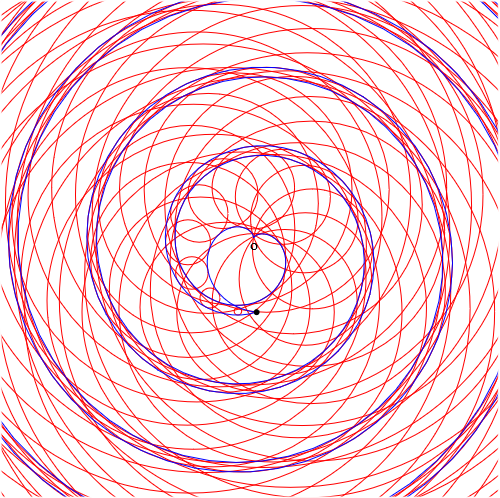
\includegraphics[width=7cm]{circular5c.png}
\caption{Same as Figure~\ref{fig:circular3c} but with $v_s=5c$.}
\label{fig:circular5c}
\end{wrapfigure}

Observers located at $r < r_s c/v_s$ do not see a shock wave and the wave frequency 
oscillates periodically as the source moves. An observer at the center, however, 
does not see any frequency change. Observers at $r>r_s c/v_s$ will be hit by shock 
waves repeatedly as the shock lines pass through them. In the case shown in 
Figure~\ref{fig:circular3c}, waves generated from multiple retarded times superpose 
in the region bounded the two shock lines, but only a single retarded time contributes 
to the wave in the region outside the shock lines. However, things can become complicated 
when $\beta_s$ increases. As shown in Figure~\ref{fig:circular5c}, waves 
generated from multiple retarded times can superpose at any location with $r > r_s c/v_s$. 
In addition, the inner shock line $Z_{\rm shock}^-$ cross itself close to the 
source location $\ve{x}_s$. So 
there are places where two shocks collide!

\end{document}
